\chapter{Ergebnisse} \label{chpt:Ergebnisse_Main}
In diesem Kapitel werden umfassend Beobachtungen präsentiert, die eine detaillierte Bewertung der Leistung und Charakteristika des entwickelten Modells ermöglichen. Die Beobachtungen erstrecken sich über verschiedene Aspekte, einschließlich der Modellleistung nach dem Training, der Qualität der generierten Bilder sowie der Schnelligkeit und Qualität von Angriffen auf das Modell.
\section{Modellleistung}
Im Folgenden werden Metriken dargestellt und verglichen, mit Hilfe derer die Leistung der verschiedenen Modelle nach Abschluss der Trainingsroutinen bewertet werden kann.
\begin{figure}[H]
	\centering
	\begin{subfigure}[b]{0.35\linewidth}
		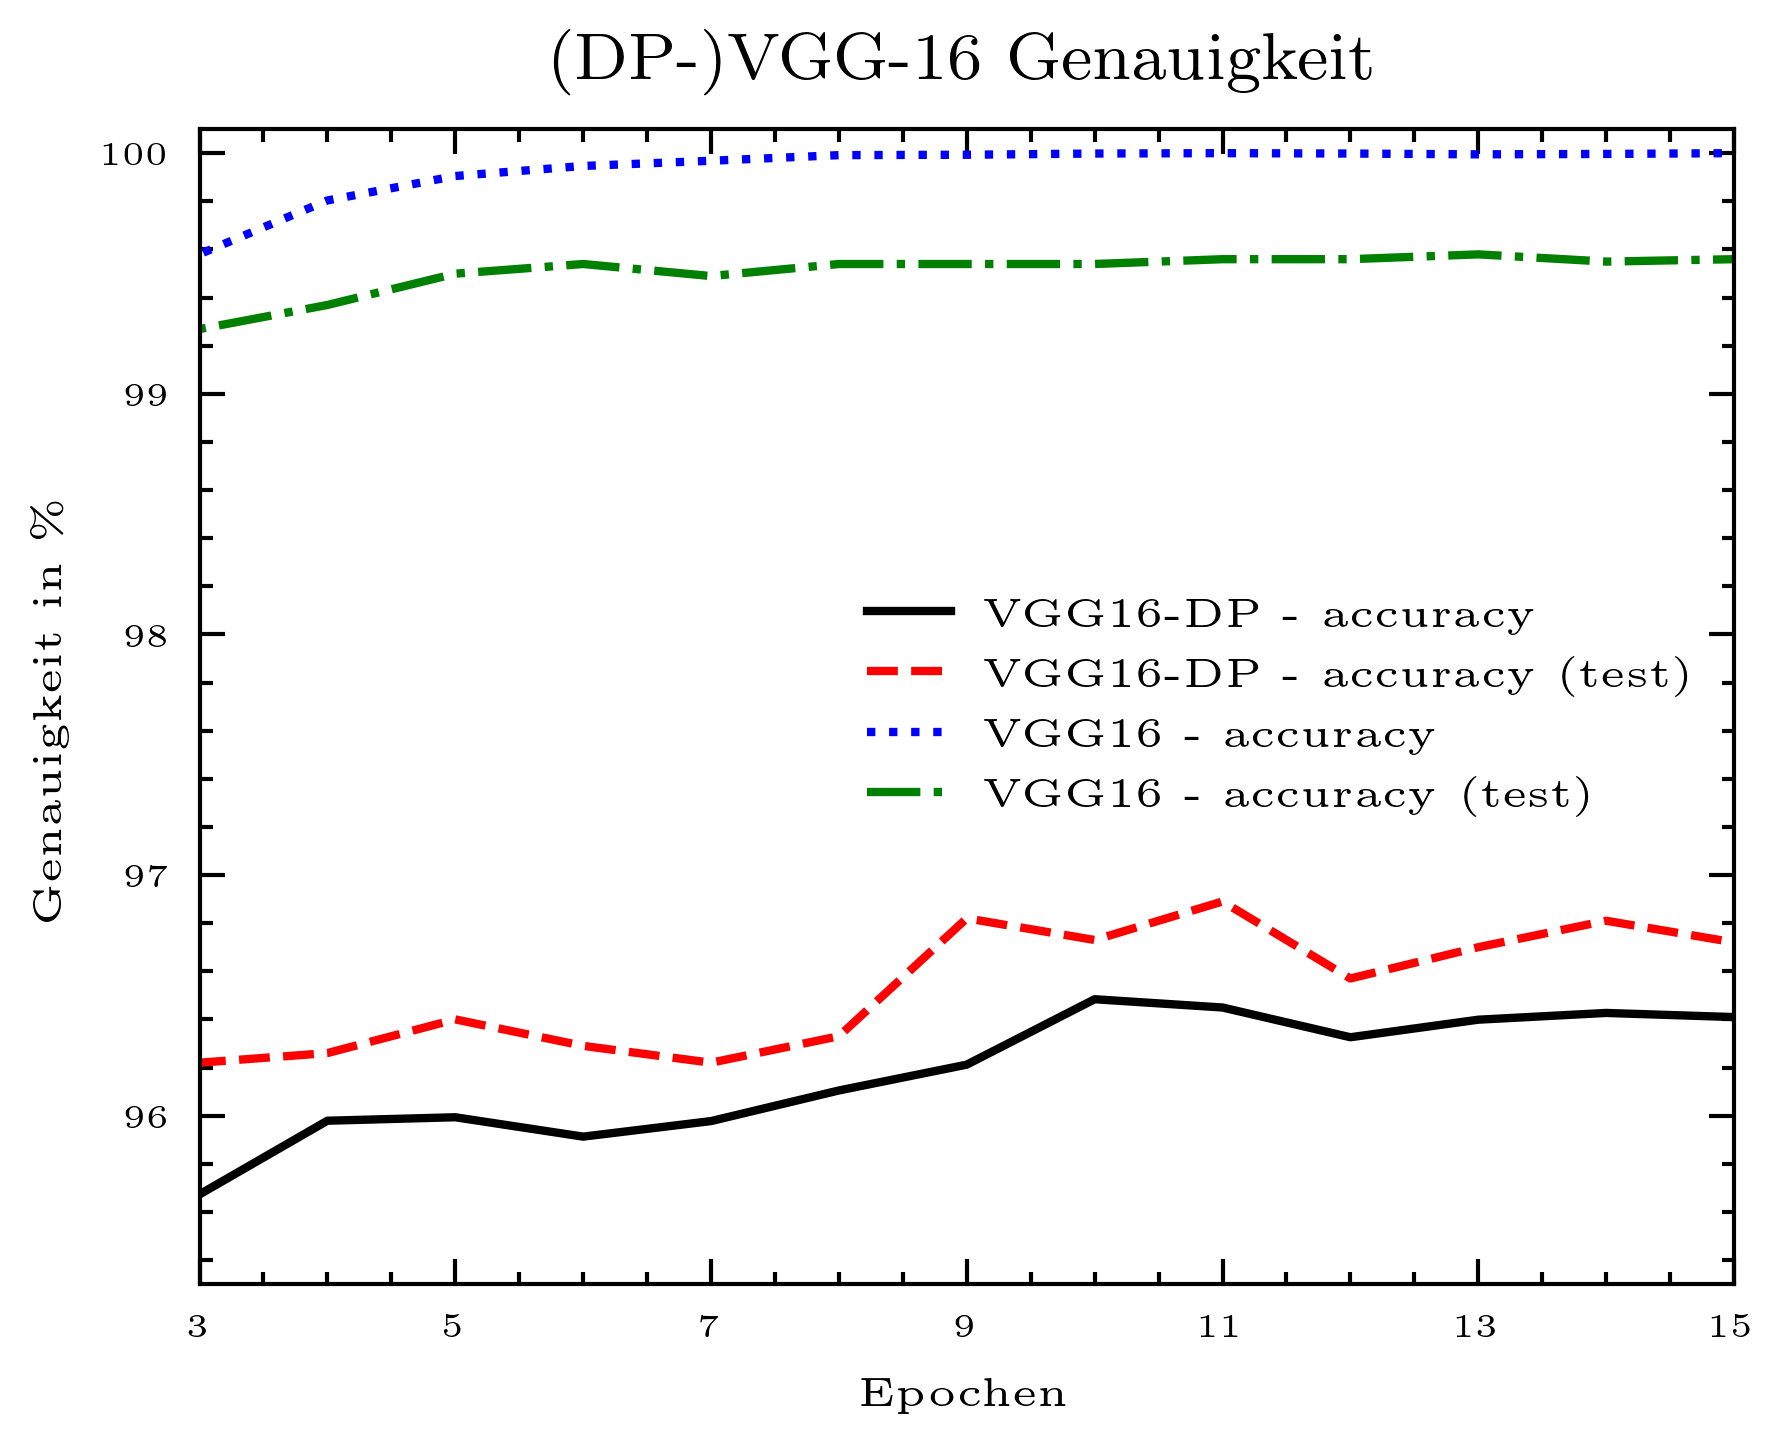
\includegraphics[width=\linewidth, height=4cm]{Bilder/acc.png}
		\caption{Modell-Genauigkeit}
		\label{img:acc_vgg_dp}
	\end{subfigure}
	\hspace{1cm} % Einfügen von horizontalen Abständen zwischen den Bildern
	\begin{subfigure}[b]{0.35\linewidth}
		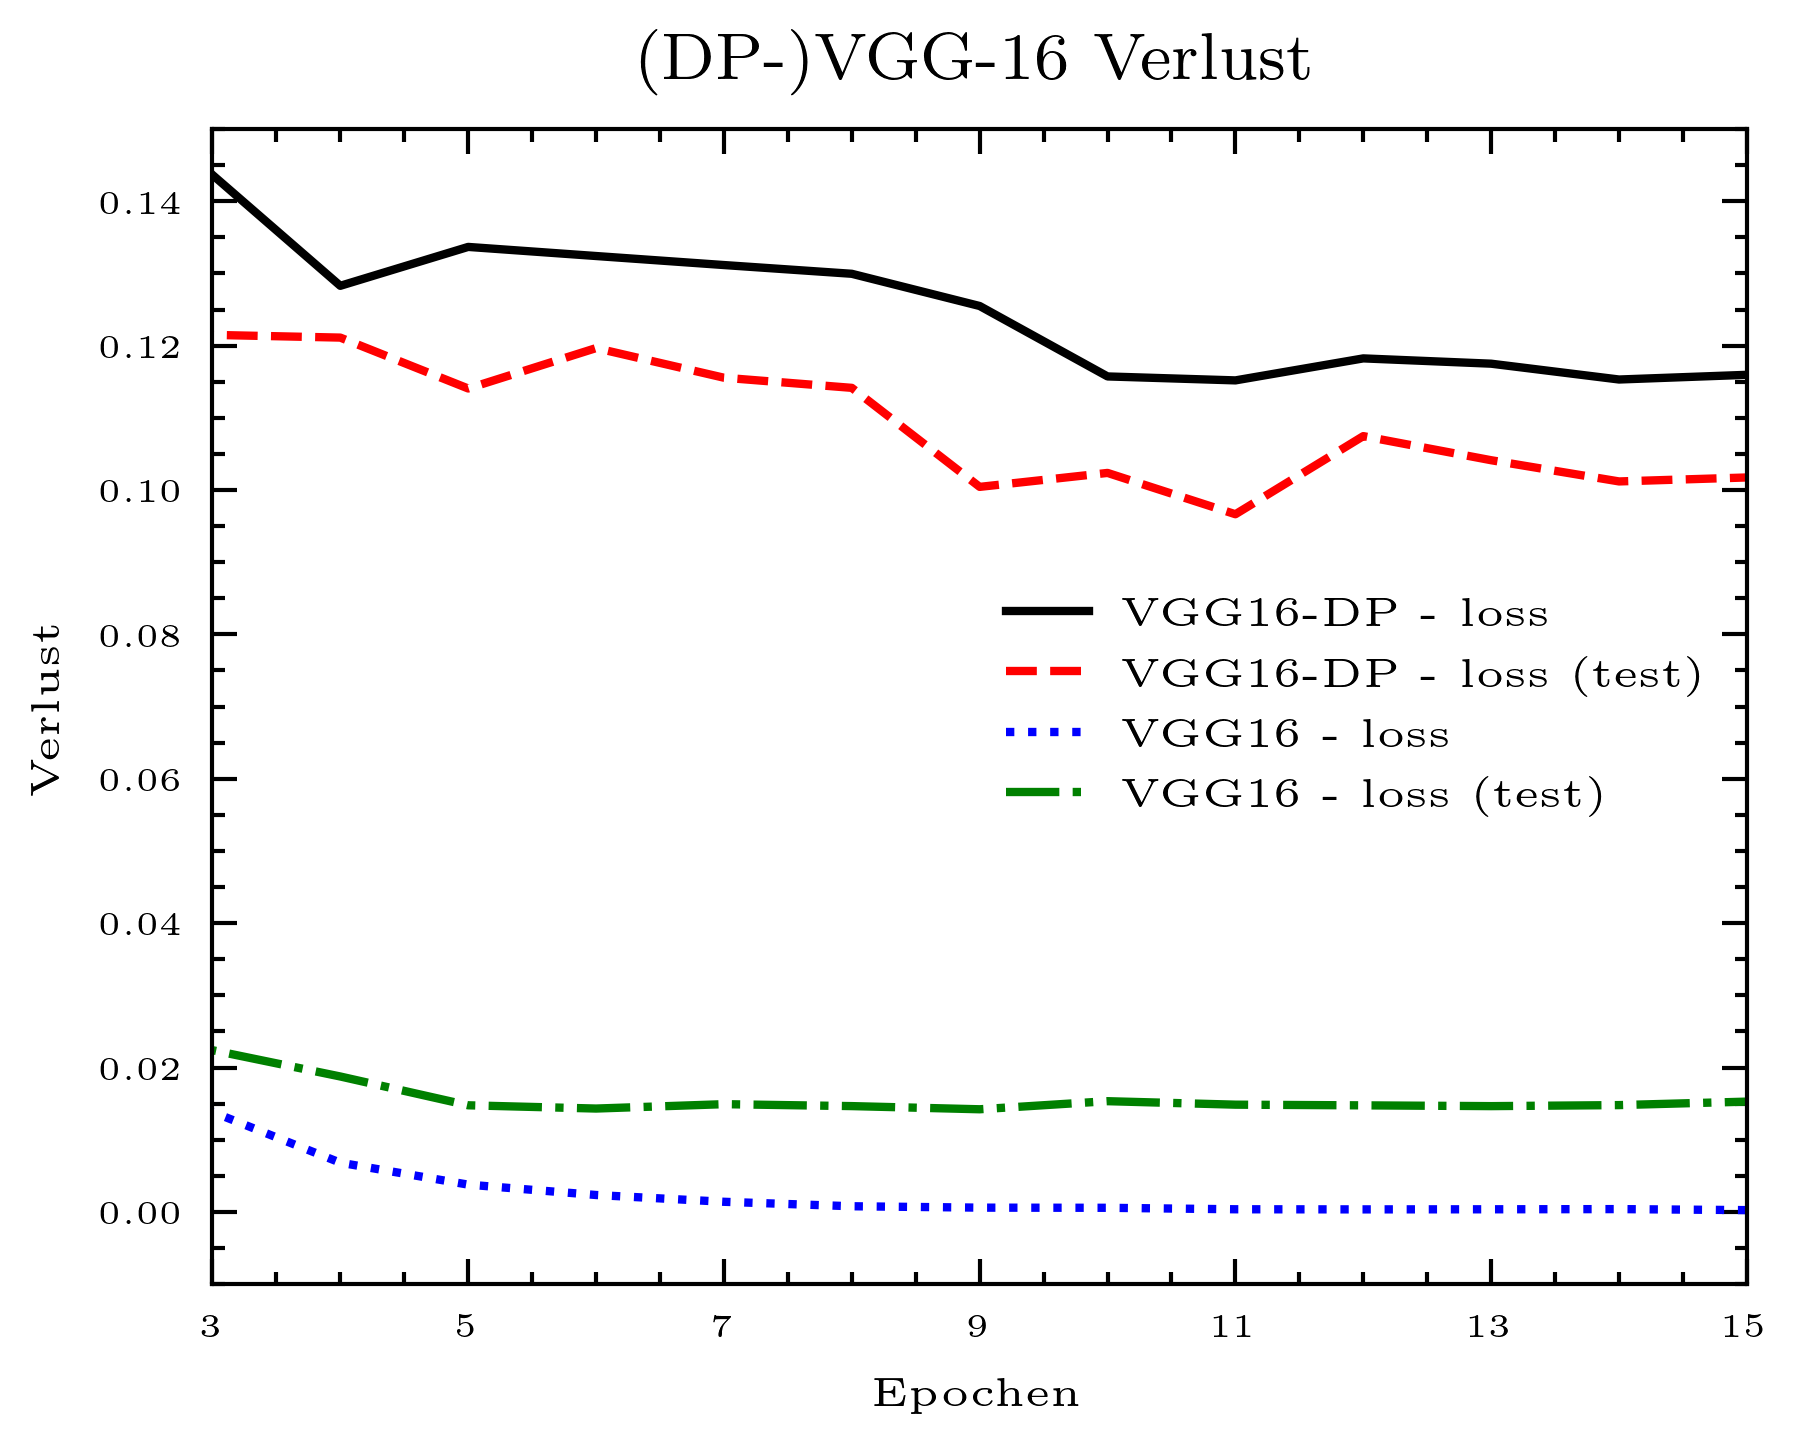
\includegraphics[width=\linewidth, height=4cm]{Bilder/loss.png}
		\caption{Verlust}
		\label{img:loss_vgg_dp}
	\end{subfigure}
	\caption{Verlust- und Genauigkeitsgegenüberstellung eines auf den MNIST-Datensatz normal und privat trainierten Modells}
	\label{img:mnist_figure}
\end{figure}
Die \textit{Genauigkeit} (\(Acc\)) (Bild \ref{img:acc_vgg_dp}) bezüglich der Test- und Trainingsdaten nimmt -- wie erwartet -- im Laufe des Trainingsprozesses zu. 
Diese wird wie folgt definiert: 
\begin{equation}
	Acc = \frac{\text{Anzahl der korrekten Vorhersagen}}{\text{Anzahl der gesamten Vorhersagen}}
\end{equation}
Während das \glqq normale Training\grqq{} mit einer Test-Genauigkeit \(Acc_{\text{test}}\) $\approx99{,}0\%$ startet und bei  \(Acc_{\text{test}}\)$\approx 99{,}5\%$ nach etwa 7 Epochen stagniert, erreicht das \glqq neuronale Netzwerk mit differentieller Privatsphäre\grqq{} zu Beginn einen deutlich niedrigeren Wert von ungefähr $91{,}5\%$ (\(Acc_{\text{test}}\)) und stagniert während der trainierten 15 Epochen noch nicht. Dabei ist allerdings zu Vermuten, dass die Genauigkeit während weiteren Epochen ansteigt, was aufgrund begrenzter Ressourcen nicht getestet werden konnte. Die hohe Genauigkeit des \glqq normalen\grqq{} Modells nach nur einer Trainingsepoche ist auf das Transfer-Learning zurückzuführen, wobei Gewichtungen anhand eines anderen, großen Datensatzes vortrainiert sind, und nicht mit Trainingsstart neu initialisiert werden müssen. 

Der \textit{Verlust} (Bild \ref{img:loss_vgg_dp}) während des Trainings zeigt einen ähnlichen Verlauf wie die oben beschriebene Test-Genauigkeit der beiden Modellarten. Nach etwa 7 Epochen beginnt dieser bei der Durchführung des \glqq normalen Trainings\grqq{} zu konvergieren und deutet darauf hin, dass das Training erfolgreich durchgeführt wurde. Im Gegensatz dazu ist wiederum bei dem \glqq Modell mit differentieller Privatsphäre\grqq{} zu beobachten, dass eine Konvergenz der Verlustfunktion nach 15 Epochen nicht erkannt werden kann. Auch hier -- wie bei Test-Genauigkeit -- lässt sich vermuten, dass eine Erhöhung der Trainingsdurchläufe eine Minimierung der Verlust-Funktion herbeiführt.  Zudem lässt sich bei beiden Modellen aus dem Verlauf der Verlustfunktion ableiten, dass die Modelle keine Überanpassung bezügliche der Trainingsdaten vorweisen. 

Das \glqq normale Training\grqq{} kann aufgrund der konvergierenden Verlust- und Genauigkeitsverte nach 7 Epochen beendet werden, da die Parameter nahezu vollständig an den Datensatz (Bild \ref{img:mnist_figure} - MNIST) angepasst sind. Dahingegen sollte man aufgrund der unvollständigen Parameteranpassung im Modell mit differentieller Privatsphäre die Anzahl der Epochen  erhöhen.

\section{Bildqualität}
Aufgrund der verschiedenen Angriffs-Verfahren variiert die Genauigkeit der Bilder in den unterschiedlichen Durchgängen, wobei die Qualität - abhängig von der Komplexität des Generative-Adversarial Networks - gleich ist. Die Genauigkeit des neu generierten Bildes, das aus privaten Daten abgeleitet ist, wird mit Hilfe des Confidence-Scores bezüglich Ziel-Klasse bestimmt. Im Folgenden werden einige Vergleiche über die Bildqualität nach der Ausführung des Angriffs basierend auf einem Klassifizierungsmodell für Zahlen und Gesichtern aufgezeigt.

Die \textit{Qualität} der Bilder ist abhängig von genutztem GAN (Generative adversarial network), das für die Generierung verwendet wird. Generierungen basierend auf dem DCGAN sind aufgrund geringerer Parameter, kürzerer Trainingsdauer und anderer Faktoren qualitativ nicht so hochwertig wie die des genutzten StyleGANs.

\begin{figure}[H]
	\centering
	\begin{subfigure}[b]{0.35\linewidth}
		
\includegraphics[width=\linewidth]{Bilder/0_mnist.png}
		\caption{Generierung der Zahl 0 auf Basis eines DCGAN}
		\label{img:gen_img_dcgan}
	\end{subfigure}
	\hspace{1cm} % Einfügen von horizontalen Abständen zwischen den Bildern
	\begin{subfigure}[b]{0.35\linewidth}
		
\includegraphics[width=\linewidth]{Bilder/401_celeba.png}
		\caption{Generierung einer Frau mit Hilfe eines StyleGANs}
		\label{img:gen_img_stylegan}
	\end{subfigure}
	\caption{Bildqualität der GAN-Modelle}
	\label{img:gen_img}
\end{figure}
Die Bilder des DCGAN basierten Generators sind etwas schwach mit vergleichsweise wenigen Pixeln aufgelöst (siehe Bild \ref{img:gen_img_dcgan}). Dahingegen lassen sich Bilder des StyleGAN Netzwerks in einer deutlich besseren Auflösung von bis zu 200 $\times$ 200 Pixeln generiern. Wie im Bild \ref{img:gen_img_stylegan} zu erkennen, wird die Qualität der Bilder durch die Reduktion der Pixel deutlich verschlechtert, was aber zu einer effektiveren Angriffsdauer führt. Im Gegensatz zu den generierten Ziffern handelt es sich bei den Gesichtern um 3-Kanal Bilder (RGB), weshalb diese farblich zu betrachtet sind.
\section{Angriffsperformance}
Dieses Kapitel befasst sich mit der Auswertung beider Angriffe nach der Durchführung, wobei im Folgenden ein Vergleich mit dem Ziel der Stärken- und Schwächenbeleuchtung aufgestellt wird. Um die Angriffe besser bewerten zu können, werden zum einen visuelle, aber auch metrische Daten begutachtet, wozu beispielsweise die Genauigkeit der neu generierten Bilder bezüglich der Ziel-Kategorie des \glqq angegriffenen\grqq{} Modells zählt.
\subsection{Genauigkeit der Angriffe}
Um eine präzisere Analyse der Angriffsgenauigkeit zu ermöglichen, werden neben visuellen Metriken auch numerische Kennzahlen integriert, um einen messbaren und vergleichbaren Wert zu erlangen.

Im Zuge der Durchführung eines \glqq KEDMI\grqq-Angriffs auf ein Zilemodell, das für die Klassifikation von handgeschriebenen Ziffern konzipiert ist, wurden entscheidende Erkenntnisse gewonnen, welche die potenzielle Gefahr des Angiffs verdeutlichen und die Notwendigkeit, adäquate Verteidigungsstragegien zu implementieren, unterstreichen. Im Folgenden werden verschiedene Metriken präsentiert, die im Rahmen der Evaluierung Verwendung finden und einen direkten Vergleich zu \glqq RBMI\grqq-Angriffen ermöglichen. Diese bieten Einblicke in die Wirksamkeit, Effektivität und Effizienz der Angriffe siwie die daraus resultierenden Auswirkungn auf die Sicherheits-Komponente des Zielmodells. Die detaillierte Analyse der Evaluierungsmetriken ermöglicht eine Bewertung der durch den Angriff aufkommenden Sschwachstelle. Diese Ergebnisse dienen zudem als Grundlage für die Ableitung geeigneter Schutzmaßnahmen zur Stärkung der Sicherheit und Robustheit des Modells gegenüber Inferenz-Angriffen.

Die visuelle Metrik zur Bewertung der Angriffsqualität stellt einen Vergleich der wiederhergestellten Bilder nach erfolgreicher Durchführung auf ein bestimmtes Zielmodell dar. Dafür werden 60 Bilder aus insgesamt 10 Klassen, die während des Angriffs generiert wurden, mit einer Sammlung von 60 Originalbildern der selben Klasse gegenübergestellt, um diese zu vergleichen. Das Angriffsziel besteht darin, dass Merkmale der Originalbilder visuell mit denen der generierten Bilder übereinstimmen, jedoch nicht jeder einzelne Trainings-Datenpunkt generiert wird.

\begin{figure}[H]
	\centering
	\begin{subfigure}[b]{0.35\linewidth}
		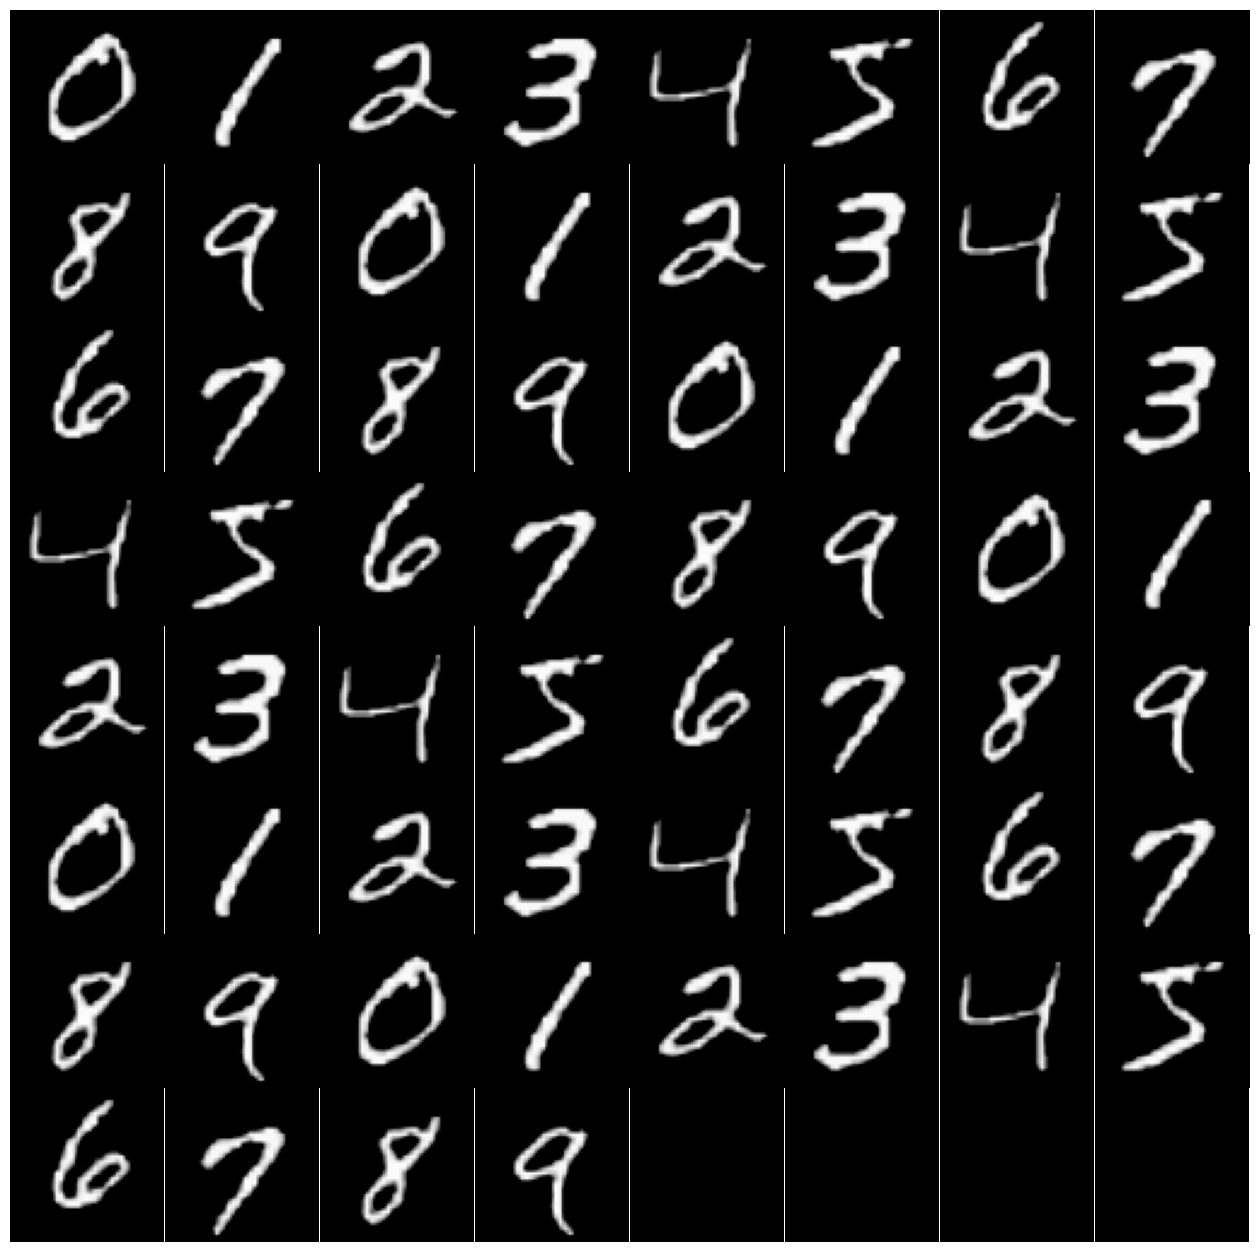
\includegraphics[width=\linewidth]{Bilder/mnist_orig.png}
		\caption{60 Originalbilder des MNIST-Datensatzes}
		\label{img:kedmi_orig}
	\end{subfigure}
	\hspace{1cm} % Einfügen von horizontalen Abständen zwischen den Bildern
	\begin{subfigure}[b]{0.348\linewidth}
		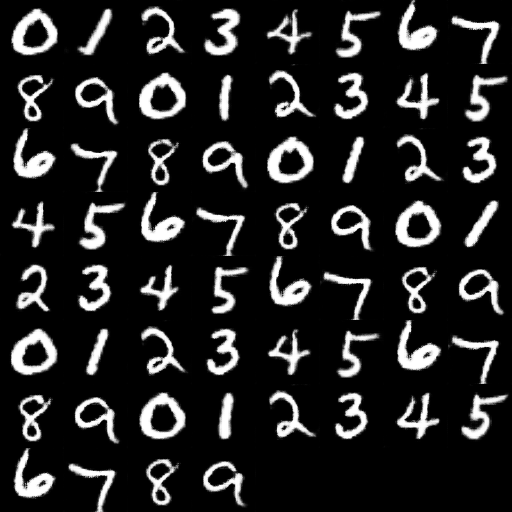
\includegraphics[width=\linewidth]{Bilder/kedmi_mnist.png}
		\caption{60 durch den \glqq KEDMI\grqq-Angriff generierte Bilder}
		\label{img:kedmi_gen}
	\end{subfigure}
	\caption{Gegenüberstellung der generierten und originalen Bilder}
	\label{img:kedmi_visual}
\end{figure}

Es zeigt sich deutlich, dass alle Klassen durch eine konsistente Übereinstimmung zwischen den originalen Bildern (siehe Abbildung \ref{img:kedmi_orig}) des Datensatzes und den generierten Bildern des \textit{"KEDMI"}-Angriffs (siehe Abbildung \ref{img:kedmi_gen}) korrekt wiederhergestellt wurden. Beim Bildvergleich wird ersichtlich, dass die Aufmachung der originalen zu den generierten Bildern variiert, was auf den Trainingsprozess und die Qualität des genutzten Generator-Netzwerks (GAN) zurückzuführen ist. Beispielsweise sind die generierten Ziffern deutlich kräftiger, als die Originalzahlen. Zudem ist erkennbar, dass die Bilder nicht exakt identisch sind, was jedoch nicht das Ziel des Angriffs darstellt, da die Bilder eine durchschnittliche Repräsentation der Features eines bestimmten Labels symbolisieren sollen.

Die visuelle Qualitätsanalyse bezüglich eines weiteren Datensatzes (CelebA) gestaltet sich aufgrund der komplexeren Datenpunktstruktur etwas unklarer im Vergleich zu den auf MNIST basierenen Angriffsgenerierungen. Die Bildqualität des verwendeten Generators (GAN) ist die komplexität der Merkmale signifikant beeinträchtigt. Auch hier werden 60 verschiedene Bilder (je eins pro Kategorie) mit dem jeweiligen Originalen der gleichen Klasse verglichen.

\begin{figure}[H]
	\centering
	\begin{subfigure}[b]{0.35\linewidth}
		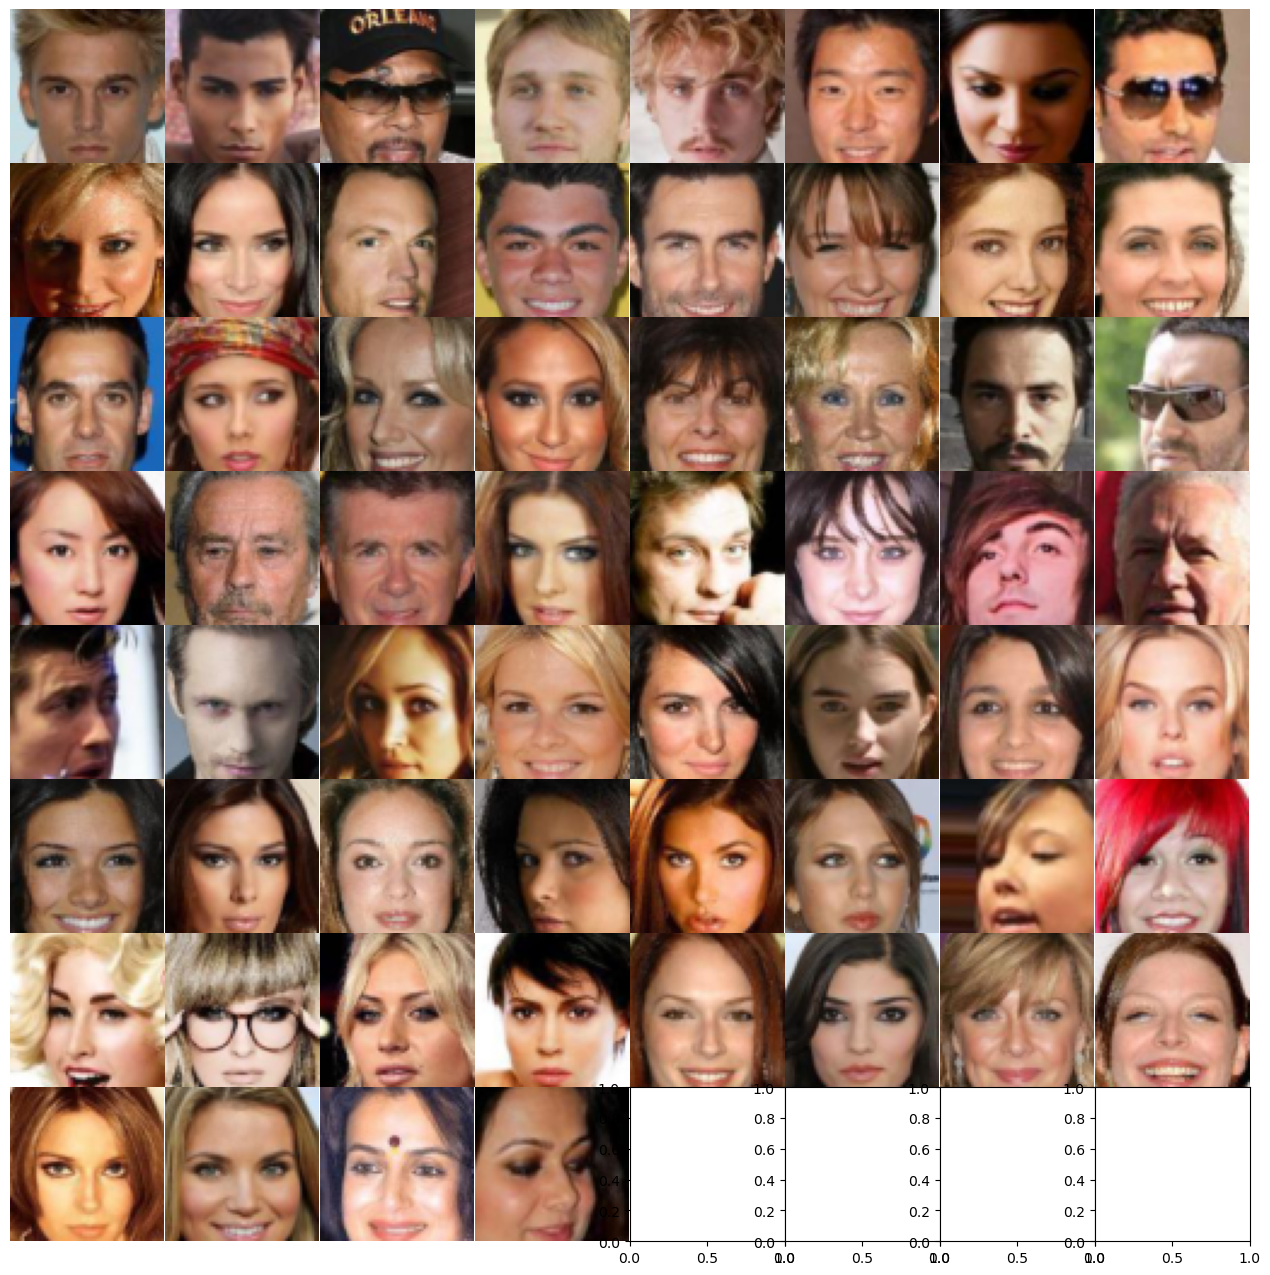
\includegraphics[width=\linewidth]{Bilder/celeba_orig.png}
		\caption{60 Originalbilder des CelebA-Datensatzes}
		\label{img:kedmi_celeba_orig}
	\end{subfigure}
	\hspace{1cm} % Einfügen von horizontalen Abständen zwischen den Bildern
	\begin{subfigure}[b]{0.348\linewidth}
		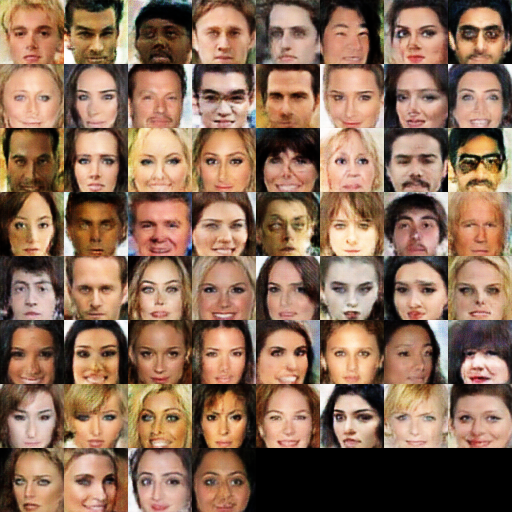
\includegraphics[width=\linewidth]{Bilder/kedmi_celeba.png}
		\caption{60 durch den \glqq KEDMI\grqq-Angriff generierte Bilder}
		\label{img:kedmi_celeba_gen}
	\end{subfigure}
	\caption{Gegenüberstellung der generierten und originalen Bilder}
	\label{img:kedmi_celeba_visuell}
\end{figure}

Bei der Durchführung des \glqq KEDMI\grqq-Angriffs auf einen für Gesichtsdaten trainierten Klassifizierer ist klar erkennbar, dass die zugrundeliegende Person, wenn auch teilweise verzerrt, wiederhergestellt wurde. Die Verzerrung und die daraus resultierende Ungenauigkeit in bestimmten Details sind auf die Bildqualität des generierenden Netzwerks zurückzuführen, das auch bei einfacher Generierung unabhängig von Angriffen Bildfehler einschleust. Es wird ebenfalls deutlich, dass die verschiedenen Bilder nicht vollständig mit dem Original übereinstimmen, da beispielsweise Personen in die \glqq falsche\grqq{} Richtung schauen. Dies ist darauf zurückzuführen, dass der Angriff nicht auf die eindeutige Generierung aller im Training verwendeten Datenpunkte abzielt, sondern auf ein Bild mit maximiertem Confidence-Score bezüglich der Zielklasse, damit dieses vom Klassifizierer mit hoher Sicherheit richtig erkannt wird, um darauf basierend die wichtigsten Features der jeweiligen Klasse zu symbolisieren. 

\subsection{Angriffsstatistiken}
% Genauigkeit normal
% Dauer
\section{Auswertung der Verteidigungsstrategie}
% Genauigkeit dp

\section{Rückschlüsse} \label{chpt:Ergebnisse_Rueckschluesse}
Hier sollen die Rückschlüsse stehen ...

